%%
%% Automatically generated file from DocOnce source
%% (https://github.com/hplgit/doconce/)
%%

% #define PREAMBLE

% #ifdef PREAMBLE
%-------------------- begin preamble ----------------------

\documentclass[%
oneside,                 % oneside: electronic viewing, twoside: printing
final,                   % draft: marks overfull hboxes, figures with paths
10pt]{article}

\listfiles               %  print all files needed to compile this document

\usepackage{relsize,makeidx,color,setspace,amsmath,amsfonts,amssymb}
\usepackage[table]{xcolor}
\usepackage{bm,ltablex,microtype}

\usepackage[pdftex]{graphicx}

% Packages for typesetting blocks of computer code
\usepackage{fancyvrb,framed,moreverb}

% Define colors
\definecolor{orange}{cmyk}{0,0.4,0.8,0.2}
\definecolor{tucorange}{rgb}{1.0,0.64,0}
\definecolor{darkorange}{rgb}{.71,0.21,0.01}
\definecolor{darkgreen}{rgb}{.12,.54,.11}
\definecolor{myteal}{rgb}{.26, .44, .56}
\definecolor{gray}{gray}{0.45}
\definecolor{mediumgray}{gray}{.8}
\definecolor{lightgray}{gray}{.95}
\definecolor{brown}{rgb}{0.54,0.27,0.07}
\definecolor{purple}{rgb}{0.5,0.0,0.5}
\definecolor{darkgray}{gray}{0.25}
\definecolor{darkblue}{rgb}{0,0.08,0.45}
\definecolor{darkblue2}{rgb}{0,0,0.8}
\definecolor{lightred}{rgb}{1.0,0.39,0.28}
\definecolor{lightgreen}{rgb}{0.48,0.99,0.0}
\definecolor{lightblue}{rgb}{0.53,0.81,0.92}
\definecolor{lightblue2}{rgb}{0.3,0.3,1.0}
\definecolor{lightpurple}{rgb}{0.87,0.63,0.87}
\definecolor{lightcyan}{rgb}{0.5,1.0,0.83}

\colorlet{comment_green}{green!50!black}
\colorlet{string_red}{red!60!black}
\colorlet{keyword_pink}{magenta!70!black}
\colorlet{indendifier_green}{green!70!white}

% Backgrounds for code
\definecolor{cbg_gray}{rgb}{.95, .95, .95}
\definecolor{bar_gray}{rgb}{.92, .92, .92}

\definecolor{cbg_yellowgray}{rgb}{.95, .95, .85}
\definecolor{bar_yellowgray}{rgb}{.95, .95, .65}

\colorlet{cbg_yellow2}{yellow!10}
\colorlet{bar_yellow2}{yellow!20}

\definecolor{cbg_yellow1}{rgb}{.98, .98, 0.8}
\definecolor{bar_yellow1}{rgb}{.98, .98, 0.4}

\definecolor{cbg_red1}{rgb}{1, 0.85, 0.85}
\definecolor{bar_red1}{rgb}{1, 0.75, 0.85}

\definecolor{cbg_blue1}{rgb}{0.87843, 0.95686, 1.0}
\definecolor{bar_blue1}{rgb}{0.7,     0.95686, 1}

%\setlength{\fboxsep}{-1.5mm}  % adjust cod_vpad/pro_vpad background box

%% Background for code blocks (parameter is color name)

%% pro/cod_vpad: gives some vertical padding before and after the text
%% (but has more simplistic code than _cod/pro_tight+cod/pro).
%% pro/cod_vpad can be used to enclose Verbatim or lst begin/end for code.
%% pro/cod calls _pro/cod_tight and has very little vertical padding,
%% used to enclose Verbatim and other begin/end for code.
%% (pro/cod is what the ptex2tex program could produce with the
%% Blue/BlueBar definitions in .ptex2tex.cfg.)

\newenvironment{cod_vpad}[1]{
   \def\FrameCommand{\colorbox{#1}}
   \MakeFramed{\FrameRestore}}
   {\endMakeFramed}

\newenvironment{_cod_tight}[1]{
   \def\FrameCommand{\colorbox{#1}}
   \FrameRule0.6pt\MakeFramed {\FrameRestore}\vskip3mm}
   {\vskip0mm\endMakeFramed}

\newenvironment{cod}[1]{
\bgroup\rmfamily
\fboxsep=0mm\relax
\begin{_cod_tight}{#1}
\list{}{\parsep=-2mm\parskip=0mm\topsep=0pt\leftmargin=2mm
\rightmargin=2\leftmargin\leftmargin=4pt\relax}
\item\relax}
{\endlist\end{_cod_tight}\egroup}

%% Background for complete program blocks (parameter 1 is color name
%% for background, parameter 2 is color for left bar)
\newenvironment{pro_vpad}[2]{
   \def\FrameCommand{\color{#2}\vrule width 1mm\normalcolor\colorbox{#1}}
   \MakeFramed{\FrameRestore}}
   {\endMakeFramed}

\newenvironment{_pro_tight}[2]{
   \def\FrameCommand{\color{#2}\vrule width 1mm\normalcolor\colorbox{#1}}
   \FrameRule0.6pt\MakeFramed {\advance\hsize-2mm\FrameRestore}\vskip3mm}
   {\vskip0mm\endMakeFramed}

\newenvironment{pro}[2]{
\bgroup\rmfamily
\fboxsep=0mm\relax
\begin{_pro_tight}{#1}{#2}
\list{}{\parsep=-2mm\parskip=0mm\topsep=0pt\leftmargin=2mm
\rightmargin=2\leftmargin\leftmargin=4pt\relax}
\item\relax}
{\endlist\end{_pro_tight}\egroup}

\usepackage{minted}
\usemintedstyle{default}

\usepackage[T1]{fontenc}
%\usepackage[latin1]{inputenc}
\usepackage{ucs}
\usepackage[utf8x]{inputenc}

\usepackage{lmodern}         % Latin Modern fonts derived from Computer Modern

% Hyperlinks in PDF:
\definecolor{linkcolor}{rgb}{0,0,0.4}
\usepackage{hyperref}
\hypersetup{
    breaklinks=true,
    colorlinks=true,
    linkcolor=linkcolor,
    urlcolor=linkcolor,
    citecolor=black,
    filecolor=black,
    %filecolor=blue,
    pdfmenubar=true,
    pdftoolbar=true,
    bookmarksdepth=3   % Uncomment (and tweak) for PDF bookmarks with more levels than the TOC
    }
%\hyperbaseurl{}   % hyperlinks are relative to this root

\setcounter{tocdepth}{2}  % levels in table of contents

% Tricks for having figures close to where they are defined:
% 1. define less restrictive rules for where to put figures
\setcounter{topnumber}{2}
\setcounter{bottomnumber}{2}
\setcounter{totalnumber}{4}
\renewcommand{\topfraction}{0.95}
\renewcommand{\bottomfraction}{0.95}
\renewcommand{\textfraction}{0}
\renewcommand{\floatpagefraction}{0.75}
% floatpagefraction must always be less than topfraction!
% 2. ensure all figures are flushed before next section
\usepackage[section]{placeins}
% 3. enable begin{figure}[H] (often leads to ugly pagebreaks)
%\usepackage{float}\restylefloat{figure}

% --- fancyhdr package for fancy headers ---
\usepackage{fancyhdr}
\fancyhf{} % sets both header and footer to nothing
\renewcommand{\headrulewidth}{0pt}
\fancyfoot[LE,RO]{\thepage}
% Ensure copyright on titlepage (article style) and chapter pages (book style)
\fancypagestyle{plain}{
  \fancyhf{}
  \fancyfoot[C]{{\footnotesize \copyright\ 2019, Ahmed Ammar. Released under CC Attribution 4.0 license}}
%  \renewcommand{\footrulewidth}{0mm}
  \renewcommand{\headrulewidth}{0mm}
}
% Ensure copyright on titlepages with \thispagestyle{empty}
\fancypagestyle{empty}{
  \fancyhf{}
  \fancyfoot[C]{{\footnotesize \copyright\ 2019, Ahmed Ammar. Released under CC Attribution 4.0 license}}
  \renewcommand{\footrulewidth}{0mm}
  \renewcommand{\headrulewidth}{0mm}
}

\pagestyle{fancy}


\usepackage{framed,wrapfig}

% --- begin definitions of admonition environments ---

% Admonition style "grayicon" has colored background, no frame, and an icon
% Admon "notice"
\definecolor{grayicon_notice_background}{rgb}{0.91,0.91,0.91}
% \fboxsep sets the space between the text and the box
\newenvironment{noticeshaded}
{\def\FrameCommand{\fboxsep=3mm\colorbox{grayicon_notice_background}}
 \MakeFramed {\advance\hsize-\width \FrameRestore}}{\endMakeFramed}

\newenvironment{notice_grayiconadmon}[1][Note]{
\begin{noticeshaded}
\noindent
\begin{wrapfigure}{l}{0.07\textwidth}
\vspace{-13pt}

\includegraphics[width=0.07\textwidth]{latex_figs/small_gray_notice}
\end{wrapfigure} \textbf{#1}\par
\nobreak\noindent\ignorespaces
}
{
\end{noticeshaded}
}

% Admonition style "grayicon" has colored background, no frame, and an icon
% Admon "summary"
\definecolor{grayicon_summary_background}{rgb}{0.91,0.91,0.91}
% \fboxsep sets the space between the text and the box
\newenvironment{summaryshaded}
{\def\FrameCommand{\fboxsep=3mm\colorbox{grayicon_summary_background}}
 \MakeFramed {\advance\hsize-\width \FrameRestore}}{\endMakeFramed}

\newenvironment{summary_grayiconadmon}[1][Résumé]{
\begin{summaryshaded}
\noindent
\begin{wrapfigure}{l}{0.07\textwidth}
\vspace{-13pt}
\includegraphics[width=0.07\textwidth]{latex_figs/small_gray_summary}
\end{wrapfigure} \textbf{#1}\par
\nobreak\noindent\ignorespaces
}
{
\end{summaryshaded}
}

% Admonition style "grayicon" has colored background, no frame, and an icon
% Admon "warning"
\definecolor{grayicon_warning_background}{rgb}{0.91,0.91,0.91}
% \fboxsep sets the space between the text and the box
\newenvironment{warningshaded}
{\def\FrameCommand{\fboxsep=3mm\colorbox{grayicon_warning_background}}
 \MakeFramed {\advance\hsize-\width \FrameRestore}}{\endMakeFramed}

\newenvironment{warning_grayiconadmon}[1][Avertissement]{
\begin{warningshaded}
\noindent
\begin{wrapfigure}{l}{0.07\textwidth}
\vspace{-13pt}

\includegraphics[width=0.07\textwidth]{latex_figs/small_gray_warning}
\end{wrapfigure} \textbf{#1}\par
\nobreak\noindent\ignorespaces
}
{
\end{warningshaded}
}

% Admonition style "grayicon" has colored background, no frame, and an icon
% Admon "question"
\definecolor{grayicon_question_background}{rgb}{0.91,0.91,0.91}
% \fboxsep sets the space between the text and the box
\newenvironment{questionshaded}
{\def\FrameCommand{\fboxsep=3mm\colorbox{grayicon_question_background}}
 \MakeFramed {\advance\hsize-\width \FrameRestore}}{\endMakeFramed}

\newenvironment{question_grayiconadmon}[1][Question]{
\begin{questionshaded}
\noindent
\begin{wrapfigure}{l}{0.07\textwidth}
\vspace{-13pt}
\includegraphics[width=0.07\textwidth]{latex_figs/small_gray_question2}
\end{wrapfigure} \textbf{#1}\par
\nobreak\noindent\ignorespaces
}
{
\end{questionshaded}
}

% Admonition style "grayicon" has colored background, no frame, and an icon
% Admon "block"
\definecolor{grayicon_block_background}{rgb}{0.91,0.91,0.91}
% \fboxsep sets the space between the text and the box
\newenvironment{blockshaded}
{\def\FrameCommand{\fboxsep=3mm\colorbox{grayicon_block_background}}
 \MakeFramed {\advance\hsize-\width \FrameRestore}}{\endMakeFramed}

\newenvironment{block_grayiconadmon}[1][Block]{
\begin{blockshaded}
\noindent
 \textbf{#1}\par
\nobreak\noindent\ignorespaces
}
{
\end{blockshaded}
}

% --- end of definitions of admonition environments ---

% prevent orhpans and widows
\clubpenalty = 10000
\widowpenalty = 10000

% --- end of standard preamble for documents ---


\usepackage[french]{babel}

% insert custom LaTeX commands...

\raggedbottom
\makeindex
\usepackage[totoc]{idxlayout}   % for index in the toc
\usepackage[nottoc]{tocbibind}  % for references/bibliography in the toc

%-------------------- end preamble ----------------------

\begin{document}

% matching end for #ifdef PREAMBLE
% #endif

\newcommand{\exercisesection}[1]{\subsection*{#1}}


% ------------------- main content ----------------------



% ----------------- title -------------------------

\thispagestyle{empty}

\begin{center}
{\LARGE\bf
\begin{spacing}{1.25}
Introduction à Python I : Présentation {\&} installation
\end{spacing}
}
\end{center}

% ----------------- author(s) -------------------------

\begin{center}
{\bf Ahmed Ammar (\texttt{ahmed.ammar@fst.utm.tn})}
\end{center}

    \begin{center}
% List of all institutions:
\centerline{{\small Institut Préparatoire aux Études Scientifiques et Techniques, Université de Carthage.}}
\end{center}
    
% ----------------- end author(s) -------------------------

% --- begin date ---
\begin{center}
Oct 22, 2019
\end{center}
% --- end date ---

\vspace{1cm}


\tableofcontents


\vspace{1cm} % after toc




% !split
\section{Objectifs généraux en premier}

Une partie essentielle de ce cours est de vous permettre de faire de la science par des expériences numériques et de développer des projets qui vous permettent d'étudier des systèmes complexes. Le but est d'améliorer ce que nous appelons la pensée algorithmique.

\paragraph{Algorithme}
Un ensemble fini d'instructions non ambiguës qui, étant donné un ensemble de conditions initiales, peuvent être effectuées dans une séquence prescrite pour atteindre un certain but.

% !split
\section{Situation standard que nous rencontrons quotidiennement}

La situation standard que nous rencontrons presque tous les séances de cours:

\begin{itemize}
\item Théorie + expérience + simulation est presque la norme dans la recherche et l'industrie.

\item Être capable de modéliser des systèmes complexes. Résoudre de vrais problèmes.

\item Accent la compréhension des principes fondamentaux et des lois dans les sciences.

\item Être capable de visualiser, présenter, discuter, interpréter et venir avec une analyse critique des résultats, et développer une attitude éthique saine pour son propre travail.

\item Améliorer le raisonnement sur la méthode scientifique.
\end{itemize}

\noindent
Une bonne présentation des résultats obtenus via de bons rapports scientifiques, aide à inclure tous les aspects ci-dessus.

% !split
\section{Langage Python}

\href{{http://www.python.org/}}{Python} est un langage de programmation moderne de haut niveau, orienté objet et d'usage général.

\textbf{Caractéristiques générales de Python} :

\begin{itemize}
\item Langage simple:
\begin{itemize}

  \item facile à lire et à apprendre avec une syntaxe minimaliste.

\end{itemize}

\noindent
\item Langage concis et expressif:
\begin{itemize}

  \item moins de lignes de code

  \item moins de bugs

  \item plus facile à maintenir.
\end{itemize}

\noindent
\end{itemize}

\noindent
% !split
\textbf{Détails techniques} :

\begin{itemize}
\item Typé dynamiquement:
\begin{itemize}

  \item Pas besoin de définir le type des variables, les arguments ou le type des fonctions.

\end{itemize}

\noindent
\item La gestion automatique de la mémoire:
\begin{itemize}

  \item Aucune nécessité d'allouer explicitement et désallouer la mémoire pour les variables et les tableaux de données. Aucun bug de fuite de mémoire.

\end{itemize}

\noindent
\item Interprété:
\begin{itemize}

  \item Pas besoin de compiler le code. L'interpréteur Python lit et exécute le code python directement.
\end{itemize}

\noindent
\end{itemize}

\noindent
% !split
\textbf{Avantages} :

\begin{itemize}
\item Le principal avantage est la facilité de programmation, qui minimise le temps nécessaire pour développer, déboguer et maintenir le code.

\item Langage bien conçu qui encourage les bonnes pratiques de programmation:
\begin{itemize}

  \item Modulaire et orientée objet, permet l'encapsulation  et la réutilisation de code. Il en résulte souvent un code plus transparent, plus facile à améliorer et sans bug.

  \item Documentation intégré avec le code.

\end{itemize}

\noindent
\item De nombreuses bibliothèques standards, et de nombreux packages add-on.
\end{itemize}

\noindent
% !split


\vspace{6mm}

% inline figure
\centerline{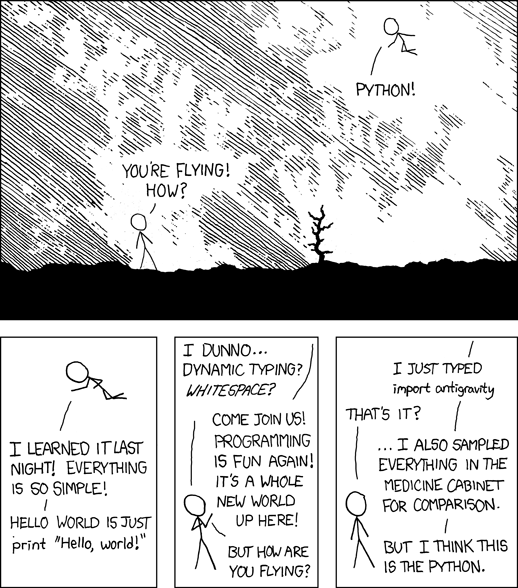
\includegraphics[width=0.6\linewidth]{imgs/python_easy.png}}

\vspace{6mm}




% !split
\section{Installation d'un environnement Python scientifique}

\subsection{Installation sur ordinateur}

\paragraph{Qu’est ce que Anaconda ?}
L’installation d’un environnement Python complet peut-être une vraie galère. Déjà, il faut télécharger Python et l’installer. Par la suite, télécharger un à un les packages dont on a besoin. Parfois, le nombre de ces librairies peut-être grand.

Par ailleurs, il faut s’assurer de la compatibilité entre les versions des différentes packages qu’on a à télécharger. Bref, ce n’est pas amusant.

% !split
\href{{https://www.anaconda.com/download/}}{Anaconda} est  une distribution Python. A son installation, Anaconda installera Python ainsi qu'une multitude de packages (voir \href{{https://docs.anaconda.com/anaconda/packages/pkg-docs#python-3-6}}{liste de packages anaconda}).  Cela nous évite de nous ruer dans les problèmes d’incompatibilités entre les différents packages.

Finalement, Anaconda propose un outil de gestion de packages appelé \href{{https://conda.io/docs/}}{conda}. Ce dernier permettra de mettre à jour et installer facilement les librairies dont on aura besoin pour nos développements.

% !split
\paragraph{Préparer la formation: téléchargement d’Anaconda.}
Nous demandons à tous les étudiants de télécharger Anaconda. Pour cela, il faut télécharger un installeur à partir de \href{{https://www.anaconda.com/download/}}{\nolinkurl{https://www.anaconda.com/download/}}, correspondant à votre système d’exploitation (Windows, Mac OS X, Linux). Il faut choisir entre 32 bits ou 64 bits (pour la version \emph{Python 3}) selon que votre système d’exploitation est 32 bits ou 64 bits.
% !split


\begin{figure}[!ht]  % 
  \centerline{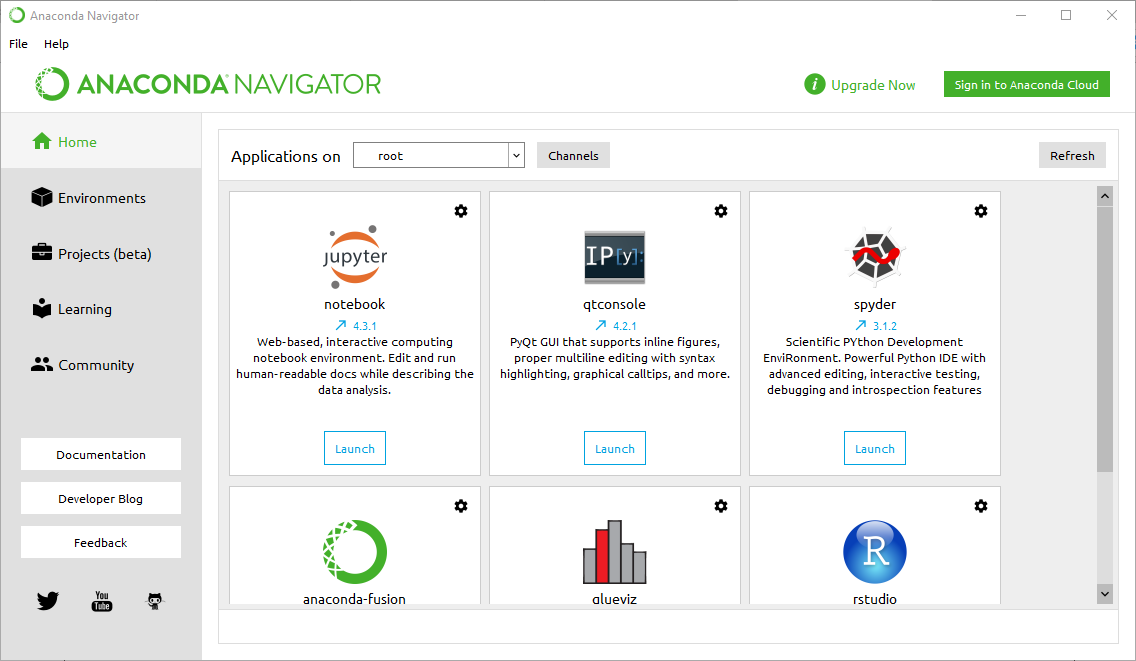
\includegraphics[width=0.7\linewidth]{imgs/AnacondaNavigator.png}}
  \caption{
  Interface graphique du navigateur Anaconda sur Windows
  }
\end{figure}
%\clearpage % flush figures 


% !split

\begin{notice_grayiconadmon}[Note]
Anaconda installe plusieurs exécutables pour développer en Python dans le répertoire \emph{anaconda/bin}, sans toujours créer des raccourcis sur le bureau ou dans un menu. Nous nous occuperons au tout début de la formation de créer des raccourcis pour pouvoir lancer l'application web \emph{Jupyter notebook}. Vous pouvez lancer le notebook depuis le navigateur Anaconda.
\end{notice_grayiconadmon} % title: Note



\subsection{Spyder}
Pour le développement de programmes en langage Python, des applications spéciales appelées IDE (Integrated Development Environment) peuvent être utilisées. Les IDE les plus avancés ont des éditeurs, des consoles, des outils pour organiser des suites de programmes et de bibliothèques, un correcteur orthographique (spell-checking) et une complétion automatiques (auto-completion) pour les scripts partiellement écrits (ces outils connaissent la syntaxe du langage de programmation) et des outils de débogage.

Utiliser un bon éditeur pour programmer en Python est bon. Utiliser un vrai IDE est encore plus confortable et puissant. \textbf{Spyder} (Scientific PYthon Development EnviRonment) semble actuellement très répandu pour l’utilisation scientifique de Python.

Spyder est un environnement de développement interactif gratuit inclus avec Anaconda. Il comprend des fonctionnalités d'édition, de test interactif, de débogage et d'introspection.

Après avoir installé Anaconda, vous pouvez démarrer Spyder sur macOS, Linux ou Windows en ouvrant une fenêtre de terminal (Ubuntu/macOS) ou d'invite de commande (Windows) et en exécutant la commande \texttt{spyder}.


\begin{figure}[!ht]  % 
  \centerline{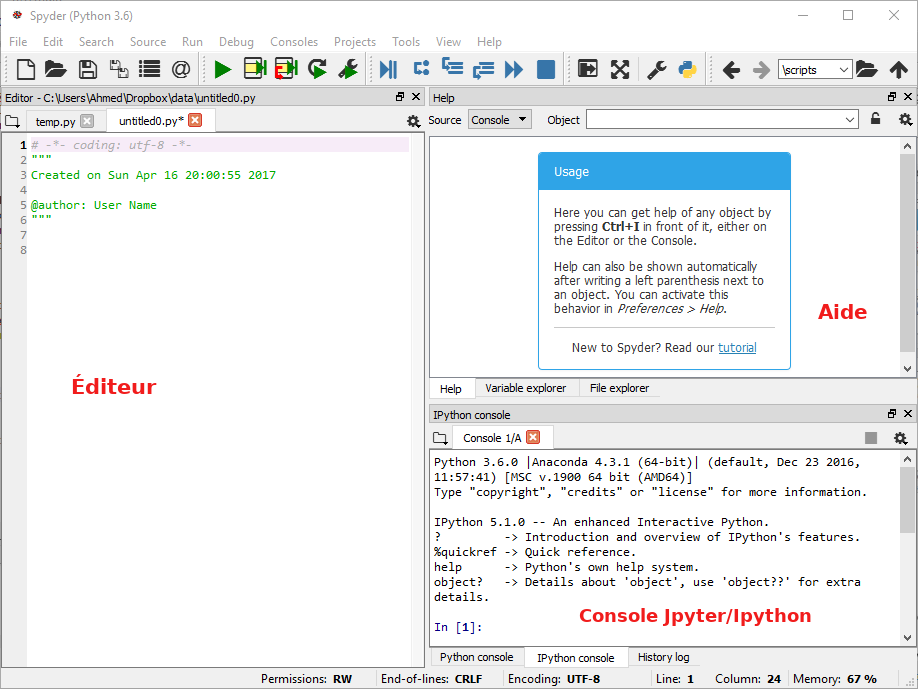
\includegraphics[width=0.7\linewidth]{imgs/SpyderIDE.png}}
  \caption{
  Spyder sous Windows.
  }
\end{figure}
%\clearpage % flush figures 


% !split
\subsection{Installation sur smartphone}

\paragraph{Pydroid 3 - IDE éducatif pour Python 3.}
Pydroid 3 est l'IDE éducatif Python 3 le plus simple et le plus puissant à utiliser pour Android.

Pydroid 3 fournit:

\begin{itemize}
\item Interpréteur Python 3.6 hors connexion: Internet n'est pas nécessaire pour exécuter des programmes Python.

\item Pip package manager et un référentiel personnalisé pour les packages de roues prédéfinis pour les bibliothèques scientifiques améliorées, tels que numpy, scipy, matplotlib, scikit-learn et jupyter.

\item ...
\end{itemize}

\noindent
% !split
\paragraph{Installer et utiliser Pydroid 3 sur son smartphone:}

Pydroid est une application Android que vous pouvez obtenir sur Google Play: \href{{https://play.google.com/store/apps/details?id=ru.iiec.pydroid3}}{\nolinkurl{https://play.google.com/store/apps/details?id=ru.iiec.pydroid3}}

Les étapes suivantes, dans les figures ci-dessous, vous permettent d’utiliser le cahier Jupyter sur votre téléphone portable n’importe où et à tout moment pour vous entraîner au maximum et vous familiariser avec tous les exemples de programmation de ce cours.

% !split
\textbf{Phase installation:}

1. Installer Pydroid 3 depuis Google Play: \href{{https://play.google.com/store/apps/details?id=ru.iiec.pydroid3}}{\nolinkurl{https://play.google.com/store/apps/details?id=ru.iiec.pydroid3}}

2. Ouvrez l'application, sur le menu cliquez sur pip et allez à l'onglet "QUICK INSTALL" pour obtenir les bibliothèques scientifiques nécessaires à ce cours.

3. Dans "QUICK INSTALL", installer les packages \emph{Jupyter} , \emph{numpy} et \emph{matplotlib}.


\begin{figure}[!ht]  % 
  \centerline{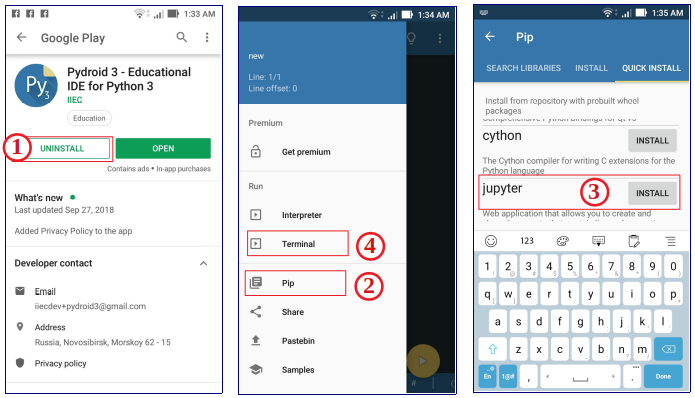
\includegraphics[width=0.7\linewidth]{imgs/pydroid3_1.png}}
  \caption{
  Pydroid 3: Phase installation
  }
\end{figure}
%\clearpage % flush figures 


% !split
\textbf{Phase utilisation:}

4. Retournez au menu et ouvrez le \textbf{terminal}.

5. Sur le terminal, entrez la commande suivante:

\begin{cod}{cbg_gray}\begin{minted}[fontsize=\fontsize{9pt}{9pt},linenos=false,mathescape,baselinestretch=1.0,fontfamily=tt,xleftmargin=2mm]{console}
jupyter notebook
\end{minted}
\end{cod}
\noindent

6. Jupyter s'exécutera sur votre navigateur Web. Accédez au répertoire dans lequel vous avez des notebooks à ouvrir, à télécharger (bouton \emph{upload}) ou à créer (bouton \emph{New}).

7. Amusez-vous à travailler sur le notebook: créez du contenu, lancez et modifiez des exemples


\begin{figure}[!ht]  % 
  \centerline{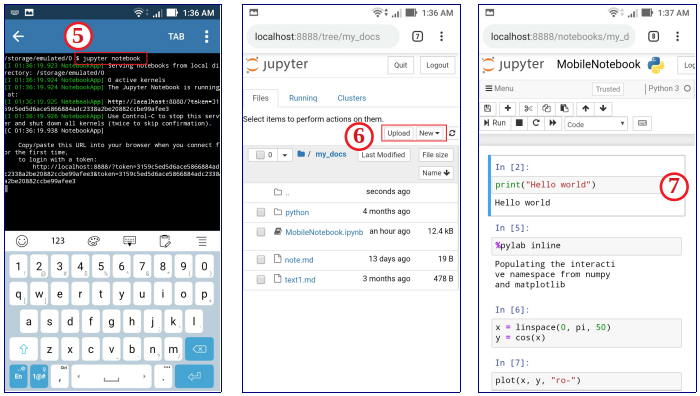
\includegraphics[width=0.7\linewidth]{imgs/pydroid3_2.png}}
  \caption{
  Pydroid 3: Phase utilisation
  }
\end{figure}
%\clearpage % flush figures 


% ------------------- end of main content ---------------

% #ifdef PREAMBLE
\end{document}
% #endif

